%% Exemple de source LaTeX pour un article soumis aux JEP 2014
\documentclass[10pt,a4paper,twoside]{article}

\usepackage[utf8]{inputenc}
\usepackage[T1]{fontenc}
\usepackage{graphicx}

% faire les \usepackage dont vous avez besoin AVANT le \usepackage{jep2014} 
% add the \usepackage for your packages BEFORE the \usepackage{jep2014}

\usepackage{hyperref}
\usepackage{amsmath}
\usepackage{pbox}
\usepackage{multirow} 
\usepackage{caption}
\usepackage{subcaption}
\usepackage{dblfloatfix} 

\usepackage{jep2014}
% Insérer les définitions de biblio en français (cf apalike-fr.bst)
\usepackage[frenchb]{babel}

\title{Combinaison de mots et de syllabes pour transcrire la parole}

\author{Luiza Orosanu\up{1, 2, 3}\quad Denis Jouvet \up{1, 2, 3}\\
{\small  Équipe PAROLE, LORIA \\
  (1) Inria, Villers-lès-Nancy, F-54600, France \\  
  (2) Université de Lorraine, LORIA, UMR 7503, Villers-lès-Nancy, F-54600, France \\ 
  (3) CNRS, LORIA, UMR 7503, Villers-lès-Nancy, F-54600, France \\ 
  \texttt{ \{luiza.orosanu, denis.jouvet\}@loria.fr} \\ 
}}

\begin{document}

\maketitle

%% In an English article, use \resumeEn with 2 arguments (French title and French summary)
\resume{
Cet article analyse l'intérêt de modèles de langage hybrides pour transcrire de la parole. 
L'objectif est d'utiliser une telle solution pour aider à la communication avec des personnes sourdes, et de la mettre en œuvre sur un terminal portable, ce qui introduit des contraintes sur la taille du modèle. 
Les unités linguistiques considérées pour cette tâche sont les mots et les syllabes. 
Des lexiques de différentes tailles sont obtenus en variant le seuil de sélection associé aux fréquences d'occurrence des mots dans les données d'apprentissage, les mots les moins fréquents sont alors décomposés en syllabes. 
Ce type de modèle de langage peut reconnaître entre 69\% et 96\% des mots (le reste étant représenté par des syllabes). En ajustant le seuil sur les mesures de confiance associées aux mots reconnus, les hypothèses de mots les plus fiables peuvent être identifiées (à un taux de bonne reconnaissance variant entre 70\% et 92\%). \\
}

%% In an English article, use \abstractEn with 1 argument (English summary)
\abstract{Combining words and syllables for speech transcription}{
\emph{This paper analyzes the use of hybrid language models for automatic speech transcription. The goal is to later use such an approach as a support for helping communication with deaf people, and to run it on an embedded decoder on a portable device, which introduces constraints on the model size. The main linguistic units considered for this task are the words and the syllables. Various lexicon sizes are studied by setting thresholds on the word occurrence frequencies in the training data, the less frequent words being therefore syllabified. Using this kind of language model, the recognizer can output between 69\% and 96\% of the words (whereas the other words, will be represented by syllables). By setting different thresholds on the confidence measures associated to the recognized words, the most reliable word hypotheses can be identified, and they have correct recognition rates between 70\% and 92\%.} \\
}

\motsClefs{modèle de langage hybride, mots, syllabes, mots hors vocabulaire, mesure de confiance, surdité}
{hybrid language model, words, syllables, out-of-vocabulary words, confidence measure, deaf people}


%% Aller à la page suivante si nécessaire
%\newpage
%%================================================================


%%%%%%%%%%%%%%%%%%%%%%%%%%%%%

\section{Introduction}

Le projet RAPSODIE porte sur l'extraction d'informations pertinentes à partir du signal de parole, afin d'aider à la communication avec des personnes sourdes ou malentendantes. Compte tenu des contraintes imposées par les ressources disponibles (capacité mémoire et puissance de calcul) avec un système embarqué, la solution optimale doit reposer sur le meilleur compromis entre coût de calcul et performance pour le modèle de reconnaissance, ainsi que sur la meilleure manière de présenter l'information reconnue (en mots, syllabes, phonèmes ou en les combinant).

Au cours des dernières décennies, les scientifiques ont essayé d'offrir une meilleure compréhension de la parole pour la communauté des sourds, en affichant des phonèmes pour aider la lecture labiale \cite{Sokol1996}, en affichant des informations en langage des signes grâce à un avatar \cite{Cox2002} et, bien entendu, en affichant des sous-titres générés d'une manière semi-automatique ou entièrement automatique. Les aspects ergonomiques et les conditions d'utilisation de la reconnaissance vocale pour aider les personnes sourdes ont été analysés dans \cite{Woodcock1997}.

L'un des principaux inconvénients des systèmes de reconnaissance de la parole est leur incapacité à reconnaître les mots qui n'appartiennent pas à leur vocabulaire. Compte tenu de la quantité limitée des données d'apprentissage, et aussi de la capacité mémoire et de la puissance de calcul limitées des systèmes de traitement, en particulier, pour des systèmes intégrés dans un dispositif portable, il est impossible de concevoir un système de reconnaissance qui couvre tous les mots, et encore moins tous les noms propres et les abréviations. Par conséquent, un système de reconnaissance grand vocabulaire (basé sur les mots) ne peut pas être une solution idéale.

IBM a ainsi testé le sous-titrage en phonétique du discours d'un orateur, avec le système appelé LIPCOM \cite{Coursant1999}. Le système de reconnaissance était mono-locuteur, et a été testé dans une école pour enfants sourds. L'application était basée sur un décodage phonétique (sans aucun vocabulaire préalablement défini) et le résultat était affiché en phonèmes codés sur une ou deux lettres. 

Toutefois, étant donné que notre objectif est de trouver une solution adaptée aux personnes sourdes et malentendantes, les priver de transcriptions basées sur des mots serait une erreur. Par conséquent, l'utilisation en complément de mots, d'unités de sous-mots, pourrait résoudre ce problème. Cela éviterait d'afficher systématiquement des informations erronées quand des mots hors vocabulaire sont prononcés; les parties hors vocabulaire seraient affichées en sous-mots. Le résultat serait alors un texte lisible et compréhensible, et la taille raisonnable du lexique limiterait les besoins en ressources de traitement.

Des études ont été menées pour étendre les lexiques de mots avec des fragments de mots, dans le but de diminuer les erreurs liées aux mots hors vocabulaire. 
La méthode proposé dans \cite{Yazgan2004} utilise un modèle de langage hybride qui combine des mots avec des unités de sous-mots tels que les phonèmes ou les syllabes. 
Une étude sur les vocabulaires ouverts a été faite aussi dans \cite{Bisani2005} où les mots et des fragments de mots ont été mélangés conjointement dans un modèle de langage hybride; les fragments de mots résultent des séquences de lettres obtenues avec les multigrammes conjoints (sequences de lettres et séquences de phonèmes). 
Dans \cite{Rastrow2009}, les unités de sous-mots correspondent à des séquences de phonèmes de longueurs variables déterminées automatiquement à partir de données; une telle extension est censée fournir des meilleures correspondances acoustiques sur les parties hors-vocabulaire du signal de parole, ce qui réduit le taux d'erreur phonétique. 
Des études plus récentes \cite{shaik2011} ont examiné la combinaison de plus de deux types d'unités lexicales dans le même vocabulaire et modèle de langage : les mots les plus fréquents sont conservés, les autres étant remplacés par des morphèmes graphémiques ou des syllabes.  

L'apport des mesures de confiance \cite{Jiang2005} dans l'emploi de transcriptions automatiques de parole pour des personnes sourdes a été analysé dans \cite{Razik2008}. Des tests subjectifs ont même montré une préférence pour l'affichage sous forme phonétique pour les mots avec une faible mesure de confiance. Cependant, le phonème présente de nombreuses irrégularités dans ses réalisations acoustiques et une unité de reconnaissance plus grande devrait être considérée pour capter les variations comme celles introduites par la coarticulation.

La syllabe a été étudiée dans le passé en tant qu'unité acoustique \cite{CerfDanon1989, Wu1998,Zhang2002, Tachbelie2011}, pour la reconnaissance de la parole continue avec un grand vocabulaire, généralement en combinaison avec des phonèmes dépendants du contexte \cite{Ganapathiraju2001, Hamalainen2005} ou pour le décodage phonétique uniquement \cite{Blouch2006}. 
Dans \cite{Wu1998}, la syllabe a été décrite comme une unité attrayante pour la reconnaissance grâce à sa plus grande stabilité, à son lien naturel entre l'acoustique et l'accès lexical et à sa capacité d'intégrer les informations prosodiques dans la reconnaissance. Dans \cite{Blouch2006}, la coarticulation a été modélisée entre les phonèmes à l'intérieur de la syllabe, mais aucune modélisation dépendante du contexte n'a été prise en compte entre les syllabes, de plus le modèle de langage appliqué au niveau de la syllabe était un bigramme.

Dans nos travaux précédents, nous avons considéré la syllabe comme une unité linguistique pour la création de modèles de langage pour un décodage phonétique \cite{Orosanu2013_1}. Même si les résultats ont montré que les meilleures performances sont toujours obtenues avec un système de reconnaissance grand vocabulaire, le choix d'utiliser un modèle de langage syllabique ne doit pas être ignoré. Il offre des performances de décodage phonétique qui sont seulement 4\% inférieures à celles fournies par le système de reconnaissance grand vocabulaire, mais nettement supérieures à celles obtenues avec un modèle phonétique et un trigram sur les phonèmes. Cela nous a conduit à considérer un modèle de langage hybride des mots et des syllabes. 

Pour se positionner par rapport aux travaux précédents, il faut préciser que nous voulons non seulement réduire les erreurs liées aux portions correspondant aux mots hors vocabulaire, mais aussi maximiser la compréhension de la transcription résultante pour la communauté de personnes sourdes. Pour ce faire, nous avons cherché à modéliser les suites de sons, plutôt que les suites de lettres. Les particularités de la langue française nous ont aussi poussé à chercher une solution qui prenne en compte la prononciation ou non du e-muet ou des phonèmes de liaison. Ce qui explique notre choix final de fabriquer des modèles de langage hybrides basés sur la transcription de prononciations de parole (au niveau mots, et au niveau phonèmes en passant par un alignement forcé). 
Par conséquent, l'objectif des travaux présentés dans cet article est de déterminer si la combinaison de mots et de syllabes (dans le lexique et le modèle de langage) conduit néanmoins à un bon taux de reconnaissance de mots. L'autre objectif est l'étude de l'apport et de la pertinence des mesures de confiance pour identifier les mots correctement reconnus. 

Le papier est organisé comme suit : la section 2 fournit une description du modèle de langage hybride, la section 3 est consacrée à la description des corpus de données et des outils utilisés dans nos expériences, et la section 4 présente et analyse les résultats.



%%%%%%%%%%%%%%%%%%%%%%%%%%%%%

\section{Contexte expérimental}

\subsection{Données}

Les corpus de parole utilisés dans nos expériences proviennent des campagnes d'évaluation ESTER2 \cite{Galliano2009} et ETAPE \cite{Gravier2012}, et du projet EPAC \cite{ESTEVE2010}.
Les données d'ESTER2 et d'EPAC sont des bulletins d'informations français recueillis auprès de diverses stations de radio, ils contiennent de la parole "préparée" et de la parole spontanée (par exemple les interviews). 
Une grande partie des données de parole sont de qualité studio, et certaines parties sont de qualité téléphonique. 
À l'inverse, les données d'ETAPE correspondent à des débats, et ont été collectées auprès de diverses chaînes de radio et de télévision. Il s'agit essentiellement de parole spontanée.

Les données de parole de l'ensemble d'apprentissage d'ESTER2 et d'ETAPE, ainsi que les données transcrites du corpus EPAC, ont été utilisées pour apprendre les modèles acoustiques. Les données d'apprentissage s'élèvent à environ 300 heures de parole et 4 millions de mots. Le modèle de langage hybride de mots et de syllabes a été appris sur les corpus des transcriptions d'ESTER2, d'ETAPE et d'EPAC (après alignement forcé).

Les variantes de prononciation ont été extraites du lexique BDLEX \cite{Calmes1998} et des lexiques internes, quand disponibles. Pour les mots manquants, les variantes de prononciation ont été obtenues automatiquement en utilisant des convertisseurs graphème-phonème JMM et CRF \cite{Illina2011}.


\subsection{Configuration}

Les modèles de langage statistiques ont été fabriqués avec les outils SRILM \cite{Stolcke2002}. 
Les outils de Sphinx3 \cite{Placeway1996} ont été utilisés pour apprendre les modèles acoustiques des phonèmes. 
Le décodage des signaux audio, ainsi que le calcul des mesures de confiance (probabilité a posteriori des mots), a été effectué avec Pocketsphinx \cite{Huggins2006}. 
L'analyse acoustique MFCC (Mel Frequency Cepstral Coefficients) donne 12 paramètres MFCC et le logarithme de l'énergie par trame (fenêtre de 32 ms, décalage de 10 ms). 
Les modèles acoustiques HMM des phonèmes utilisent des mélanges de 64 gaussiennes, et sont adaptés aux données hommes et aux données femmes. 
L'unité acoustique utilisée est toujours le phonème, avec une modélisation dépendante du contexte.

%%%%%%%%%%%%%%%%%%%%%%%%%%%%%

\section{Création du modèle de langage hybride}

La création d'un modèle de langage hybride, combinant mots et syllabes, implique de constituer un corpus d'apprentissage qui repose sur ces deux unités lexicales. Ensuite, le vocabulaire est défini en sélectionnant que les mots les plus fréquents, i.e. les mots qui apparaissent au moins $\theta$ fois dans le corpus d'apprentissage, et les mots hors vocabulaire sont décomposés en syllabes; les syllabes correspondantes sont alors ajoutées au lexique.

Un point de départ consiste à appliquer un alignement forcé sur les données d'apprentissage, afin de déterminer quelle variante de prononciation a été effectivement utilisée pour chaque mot prononcé (fréquent ou pas). À noter que les vocabulaires utilisés dans la reconnaissance de la parole peuvent avoir plusieurs variantes de prononciation, et que un ou plusieurs phonèmes peuvent manquer dans certaines d'entre elles. Ces variantes de prononciation sont nécessaires afin de tenir compte des événements de type liaison ou réduction. Ensuite, les mots peu fréquents (non sélectionnés par rapport au seuil choisi) sont remplacés par leur variante de prononciation telle que résultant de l'alignement forcé. Enfin, les séquences de phonèmes ainsi obtenues, correspondant aux segments de parole entre les mots sélectionnés, sont traitées par l'outil de syllabation, qui est basé sur les règles décrites dans \cite{Bigi2010}. Deux principes sont appliqués: une syllabe contient une seule voyelle et une pause désigne la frontière d'une syllabe.

Par exemple, dans la phrase "une femme a été blessée " : 
\begin{itemize}										 
\item[$\bullet$] mots fréquents = \{une, femme, a, été\}				
\item[$\bullet$] mot non-fréquent = \{blessée\}					
\item[$\bullet$] remplacement du mot "blessée" par sa prononciation "b l eh s e" (variante déterminée par alignement forcé) $\Rightarrow$  "une \quad femme \quad a  \quad été \quad b \quad  l \quad eh \quad s  \quad e"  
\item[$\bullet$] structuration de la séquence de phonèmes  "b l eh s e" en deux syllabes "\_b\_l\_eh" et "\_s\_e"  \vspace{0.1cm} \\
\hspace{0.1cm} \vspace{0.1cm} $\Rightarrow$  {\bf mots et syllabes :} "une \quad femme \quad a \quad été \quad  \_b\_l\_eh \quad \_s\_e".
\end{itemize}	


L'utilisation d'un modèle de langage hybride vise à assurer une reconnaissance correcte des mots les plus fréquents et à proposer des suites de syllabes pour les segments de parole correspondant à des mots hors vocabulaire. Les syllabes choisies correspondant à des suites de phonèmes, donc ayant une prononciation unique, devraient faciliter la compréhension des segments de parole hors vocabulaire, du moins plus facilement que de devoir interpréter une suite de petits mots dont l’une des variantes de prononciation correspond au segment de parole hors vocabulaire (cas fréquent lorsque le lexique et le modèle de langage n’utilisent pas d’unités sous-lexicales).


Différents seuils minimaux sur la fréquence d'occurrence des mots ont été considérés : $\theta \in \{ 3, 5, 10, 25, 50, 100, 300 \}$.
Chaque choix de seuil entraîne la création d'une transcription différente du corpus d'apprentissage (avec un nombre différent de mots et de syllabes), ce qui conduit à un lexique et un modèle de langage correspondant.


\begin{table*}[h!]
\centering
	\begin{tabular}{|c||r|r|r||r|r||r|r|r|}
	\hline
	\multirow{4}{*}{\bf Condition}  & \multicolumn{5}{c||}{\multirow{2}{*}{\bf Données d'apprentissage}}  & \multicolumn{3}{c|}{\multirow{2}{*}{\bf  Modèles de langage}} 	\\
	 & \multicolumn{5}{c||}{} & \multicolumn{3}{c|}{}  															\\ 
	\cline{2-9} 
	\cline{2-9}
	 & \multicolumn{3}{c||}{\bf \# Mots} & \multicolumn{2}{c||}{\bf \# Syllabes} & \multirow{2}{*}{\bf \# Lex} & \multirow{2}{*}{\bf \# 3g} & \multirow{2}{*}{ \pbox{3cm}{ {\bf Taille} \\ {[}MO{]} } } \\ 
	\cline{2-6}
		& {unique}  & {total} & {couv.}   & {unique} & {total} &  & & 	\\ \hline	
	{\bf min3occ}   & 31298  & 3.57 M  & 98.9\% & 2287 &  0.11 M & 33585  &  1.85 M & 14.2			\\ \hline
%	{\bf min4occ}   & 26329  & 3.55 M  & 98.5\% & 2831 &  0.15 M & 29160  &  1.85 M & 14.0			\\ \hline
	{\bf min5occ}   & 23052  & 3.54 M  & 98.1\% & 3209 &  0.19 M & 26261  &  1.86 M & 13.9	 		\\ \hline
	{\bf min10occ}  & 15052 & 3.49 M  & 96.7\% & 4050 &  0.33 M & 19102  &  1.87 M & 13.5	 		\\ \hline
	{\bf min25occ}  &  8179  & 3.38 M  & 93.8\% & 4739 &  0.62 M & 12918  &  1.86 M & 12.8	 		\\ \hline
	{\bf min50occ}  &  4895  & 3.27 M  & 90.6\% & 5126 &  0.91 M & 10021  &  1.83 M & 12.3	 		\\ \hline
	{\bf min100occ} &  2868 & 3.13 M  & 86.7\% & 5391 & 1.27 M  &  8259   &  1.79 M & 11.6	 		\\ \hline
%	{\bf min200occ} &  1553 & 2.94 M  & 81.6\% & 5619 & 1.72 M  &  7172   &  1.73 M & 10.9	 		\\ \hline
	{\bf min300occ} &  1066 & 2.83 M  & 78.3\% & 5730 & 1.99 M &  6796    &  1.69 M & 10.5			\\ \hline
	\end{tabular}
\caption{Description des modèles de langage hybrides} \label{Tab:LMs}
\end{table*}

Les différentes transcriptions et les modèles de langage associés sont décrits dans le tableau \ref{Tab:LMs}. En ce qui concerne les lexiques, les nombres d'entrées uniques (mots d'une part, et syllabes d'autre part) sont mentionnés dans le tableau. Chaque mot dans le lexique correspond à environ deux variantes de prononciation (essentiellement du fait des liaisons possibles et de la présence ou non de e-muet). Étant donné que les syllabes correspondent à une seule séquence de phonèmes, elles ne peuvent avoir qu'une seule prononciation possible \cite{Orosanu2013_1}. Le tableau indique aussi le nombre total d’occurrences des mots fréquents et des syllabes fréquentes dans le corpus d’apprentissage, ainsi que le taux de couverture avec les mots fréquents.

Les modèles de langage utilisées dans notre étude sont des modèles statistiques trigrammes, donc pour chaque séquence de trois unités lexicales, la probabilité de la dernière unité lexicale dépend de l'identité des deux unités qui la précèdent.

Pour compléter la description des modèles, seules les syllabes observées au moins trois fois dans le corpus d’apprentissage sont conservées dans les lexiques et dans les modèles de langage.


%%%%%%%%%%%%%%%%%%%%%%%%%%%%%

\section{Résultats et discussions}

Les ensembles de développement d'ESTER2 (excepté les radios africaines, soit environ 42,000 mots) et d'ETAPE (environ 82,000 mots) sont utilisés dans les expériences rapportées ci-dessous.

Étant donné que les modèles de langage mélangent des mots et des syllabes, et que nous sommes intéressés à récupérer le message porté par la parole, nous avons particulièrement analysé combien de mots ont été produits par le décodeur (dans la séquence de mots et de syllabes), et parmi ces mots, combien d’entre eux ont été effectivement bien reconnus.

Les résultats pour le corpus ETAPE sont affichés dans le tableau \ref{Tab:RecWords} : le modèle de langage qui combine les mots vus au moins 3 fois avec les syllabes vues au moins 3 fois ("min3occ") génère environ 67K mots (couvrant 96,40\% d'unités générées par le décodeur), dont 47K ont été bien reconnus (70,03\%). Avec le modèle de langage qui combine les mots vus au moins 300 fois et les syllabes vues au moins trois fois ("min300occ"), 71,11\% des hypothèses mots sont correctes, mais le nombre de mots reconnus est plus faible (53K, couvrant 68,58\% d'unités générées par le décodeur). 
Pour ESTER2, les pourcentages de mots générés par le decodeur sont similaires aux valeurs obtenues pour ETAPE (une moyenne d'environ 83\%). Cependant, les pourcentages de mots bien reconnus sont un peu plus élevés (73\%) .

\begin{table}[b!]
\begin{center}
\begin{tabular}{|c||r|r|r||r|r|}
\hline
\multirow{2}{*}{\bf ML}  & \multicolumn{3}{c||}{\bf Unités en sortie du décodeur} & \multicolumn{2}{c|}{\bf Mots corrects}  	\\ \cline{2-6}
 & {\bf \# mots} & {\bf \# syllabes} &  {\bf \% mots } & {\bf nombre} & {\bf pourcentage} 			\\ \hline\hline	
{\bf min3occ}     &  66568  &  2485   & 96.40  & 46616  & 70.03     		\\ \hline
{\bf min5occ}     &  66085  &  3787   & 94.58  & 46397  & 70.21    		\\ \hline
{\bf min10occ}   &  65293  &  5841   & 91.79  & 46111  & 70.62	 	\\ \hline
{\bf min25occ}   &  62325  &  9710   & 86.52  & 44195  & 70.91 		\\ \hline
{\bf min50occ}   &  61627  & 14405  & 81.05  & 43795  & 70.92 		\\ \hline
{\bf min100occ} &  59322  & 19507  & 75.25  & 42134  & 71.03   		\\ \hline
{\bf min300occ} &  53542  & 31605  & 68.58  & 38075  & 71.11 	  	\\ \hline
\end{tabular}
\caption{Statistiques sur les séquences d’unités en sortie du décodeur pour le corpus ETAPE : nombre de mots et de syllabes, taux d'unités mots, et statistiques sur mots bien reconnus} 
\label{Tab:RecWords}
\end{center}
\end{table}


Il est intéressant  de filtrer les mots reconnus (fournis pas le décodeur) selon leurs mesures de confiance, afin de maximiser le pourcentage de mots qui sont corrects, i.e. bien reconnus par le système (MBR, "mots bien reconnus"). Le rapport MBR est calculé comme suit: 
$$MBR(seuil)=\frac{\text{\# mots : bien reconnus \& MC} \ge \text{seuil}}{\text{\# mots : MC} \ge \text{seuil}}$$

\begin{figure*}[t!] 
\centering
        \begin{subfigure}[b]{0.45\textwidth}
		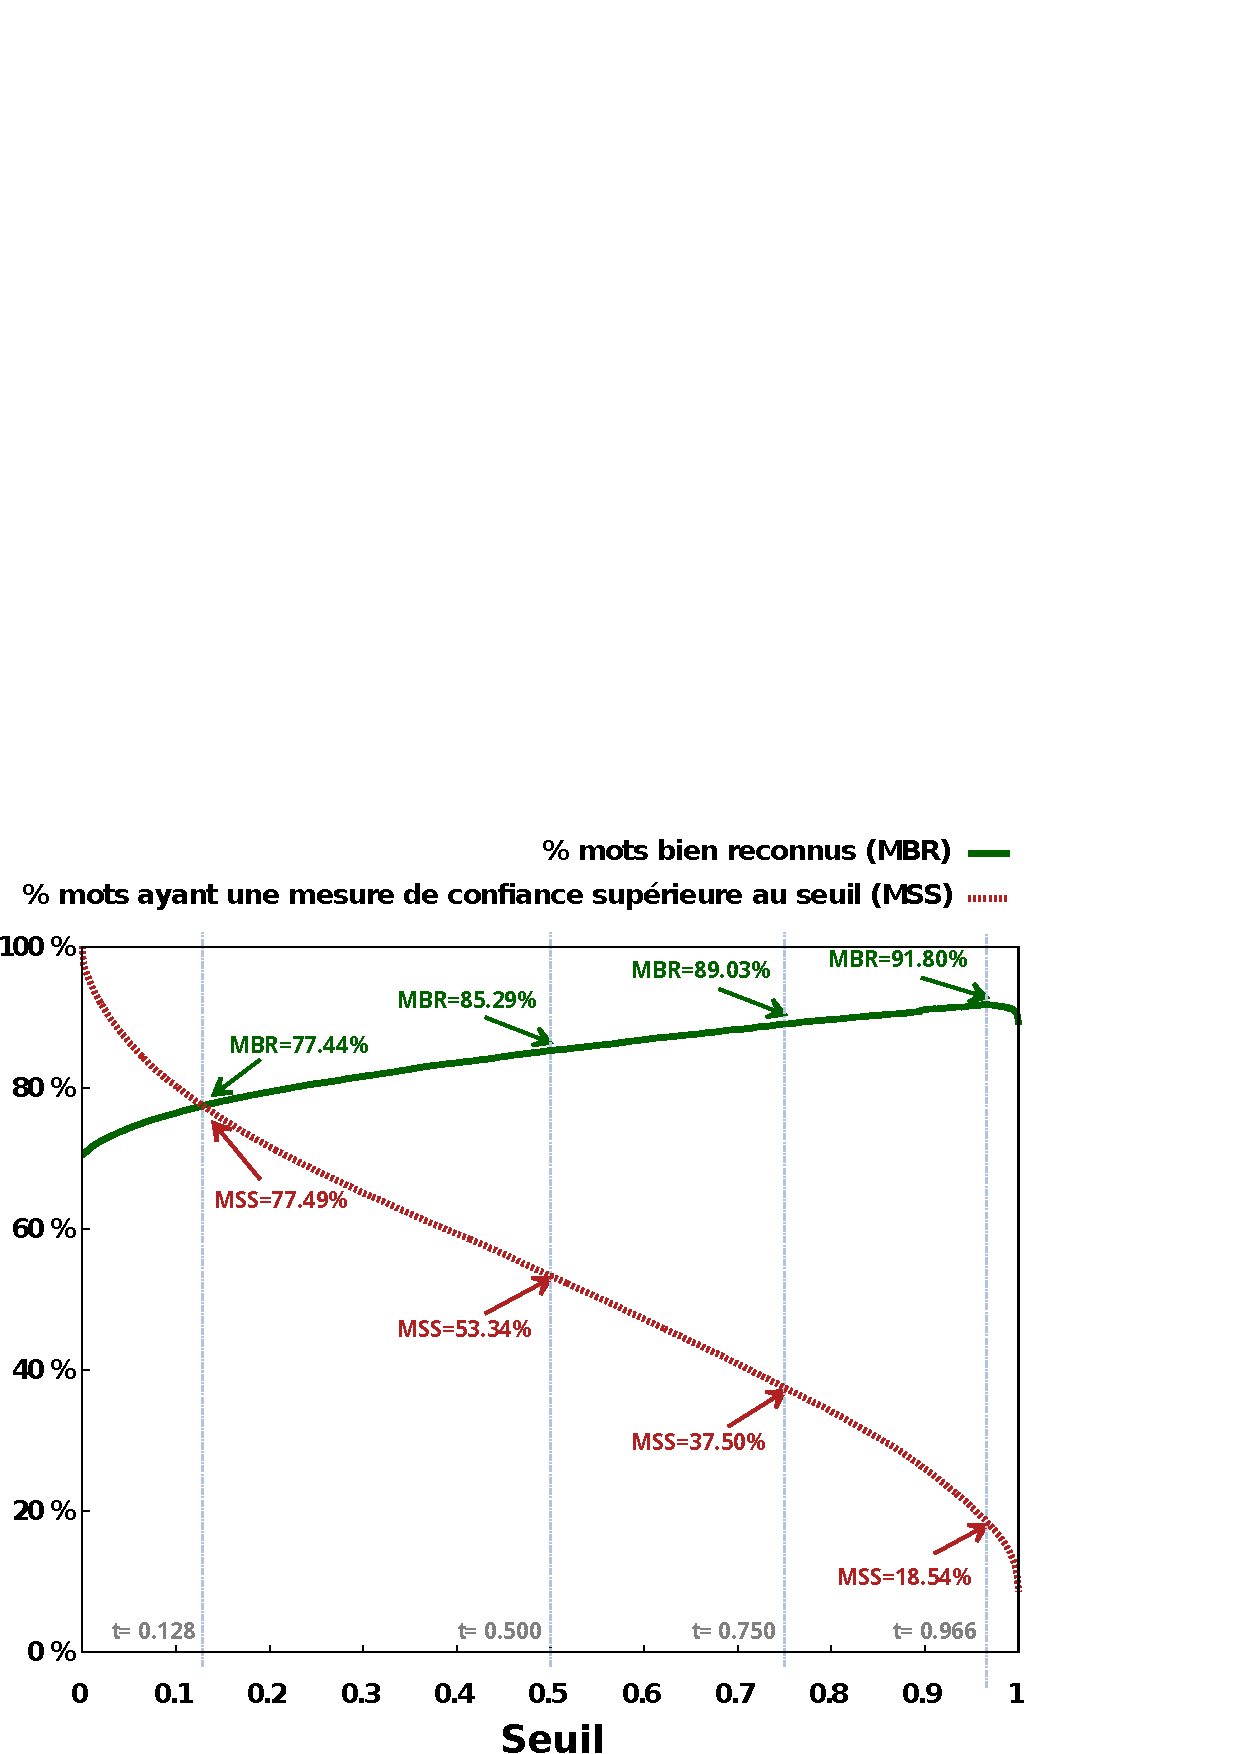
\includegraphics[scale=0.365]{Image/combined_min3occ_ETAPE.pdf}
               	\caption{Corpus = ETAPE , ML = min3occ}
        \end{subfigure}
	\hspace{0.3cm}
	\begin{subfigure}[b]{0.45\textwidth}
		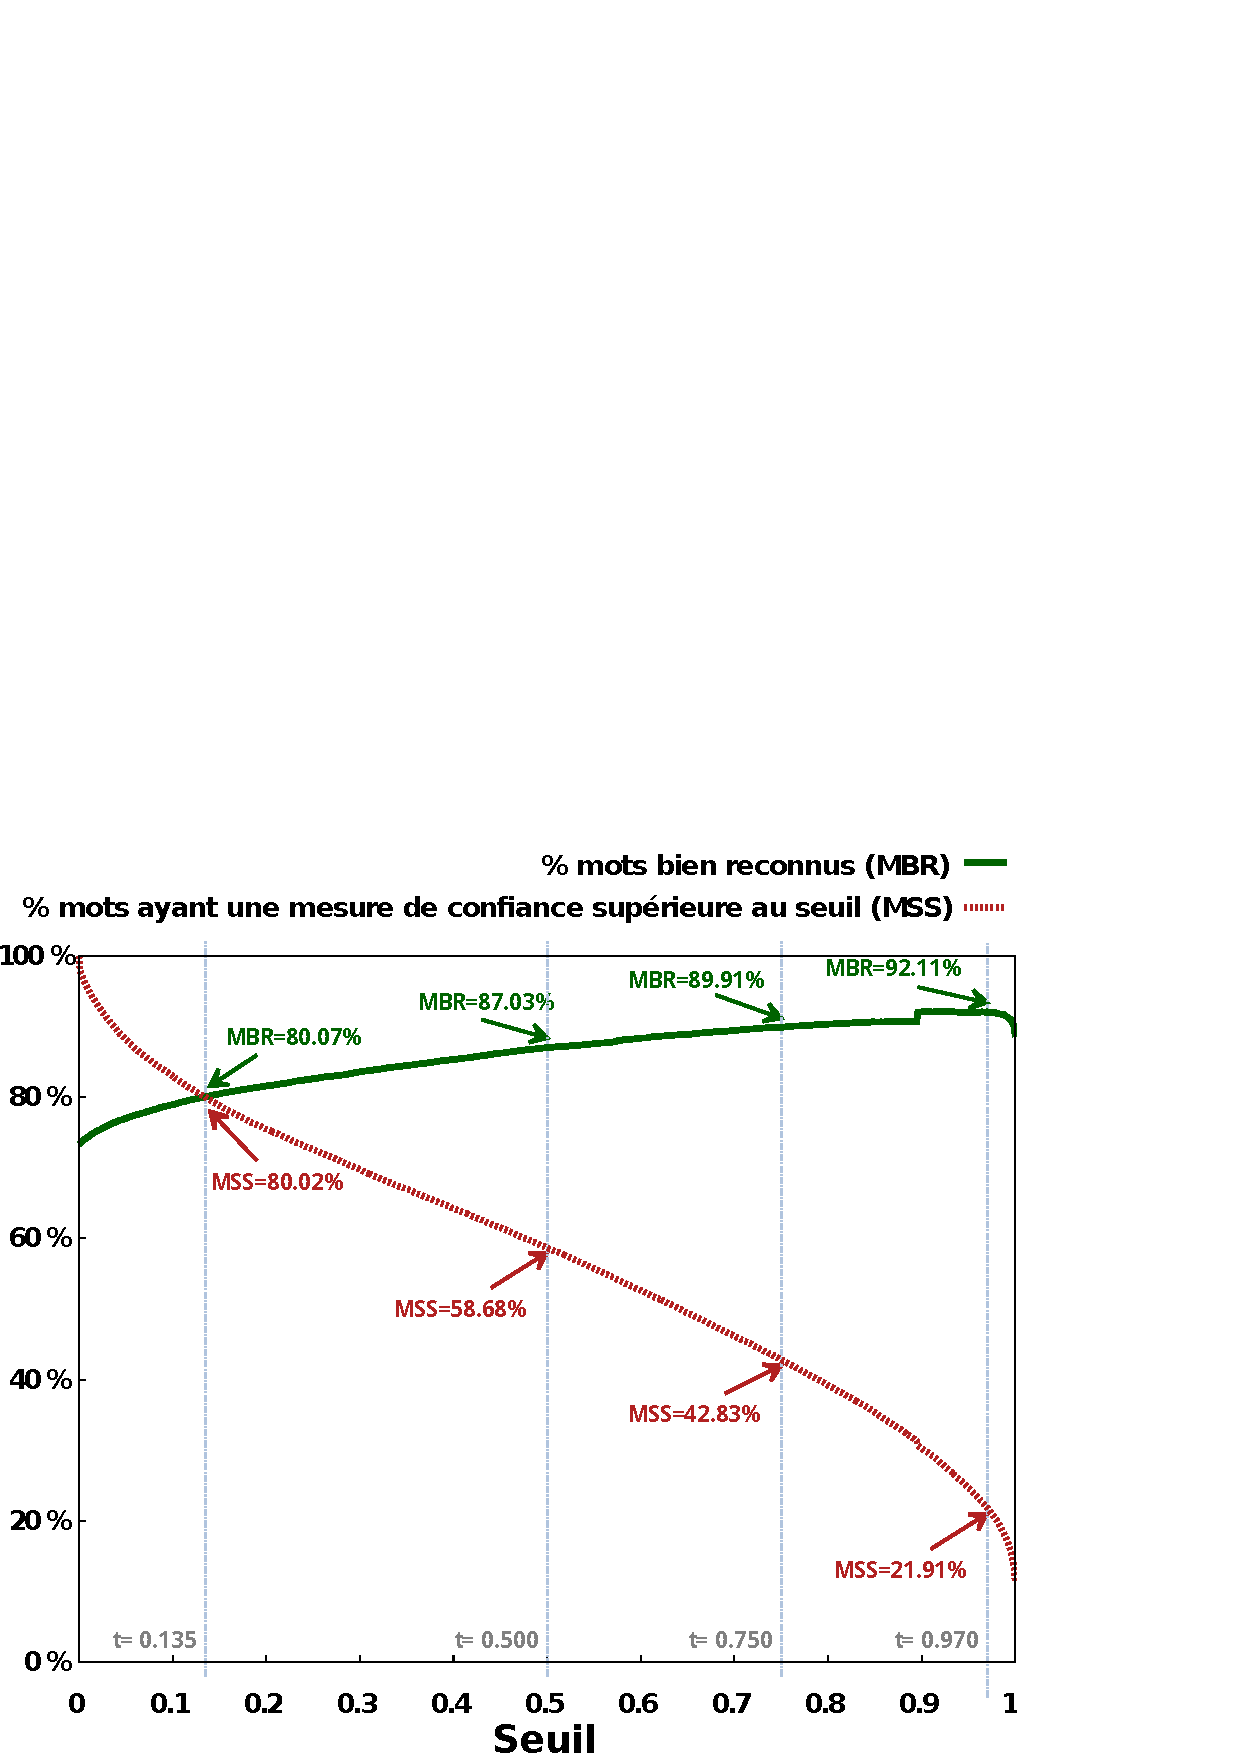
\includegraphics[scale=0.365]{Image/combined_min3occ_ESTER.pdf}
                \caption{Corpus = ESTER , ML = min3occ}
        \end{subfigure}
\caption{Analyse de l'impact du seuil pour l'acceptation de mots, basée sur leurs mesures de confiance: les courbes rouges (MSS) indiquent le pourcentage de mots ayant une mesure de confiance supérieure au seuil, et les courbes vertes (MBR), le pourcentage de ceux bien reconnus}
\label{Fig:tc}
\end{figure*}



La figure \ref{Fig:tc} montre les performances obtenues par la mise en place de divers seuils sur les mesures de confiance, en utilisant le modèle de langage "min3occ" sur le corpus ETAPE (a) et sur le corpus ESTER (b) (les résultats obtenus avec les autres modèles de langage sont similaires). 
Un seuil supérieur à 0,96 sur les mesures de confiance conduit à un ratio de mots bien reconnus supérieur à 90\% pour les deux corpus. 
Cependant, un grand seuil rejette de nombreuses hypothèses de mots (par exemple, 80\% des hypothèses de mots ont une mesure de confiance inférieure au seuil de 0.96).
L’augmentation du seuil réduit le nombre de mots conservés, mais augmente la pertinence des hypothèses conservées. 
En pratique, un compromis doit être fait entre le nombre de mots qui sont rejetés, et la performance qui peut être obtenue sur les mots non rejetés. 

Les mesures de confiance sur les syllabes semblent moins pertinentes; avec le modèle de langage "min3occ", environ 50\% des syllabes ont une mesure de confiance inferieure à 0,07.

%%%%%%%%%%%%%%%%%%%%%%%%%%%%%

\section{Conclusions}

Cet article a analysé l'intérêt de modèles de langage hybrides pour transcrire de la parole, dans le but d'utiliser une telle solution pour aider à la communication avec des personnes sourdes, et de la mettre en œuvre sur un terminal portable.
L'objectif était de déterminer si la combinaison de mots et de syllabes (dans le lexique et le modèle de langage) conduit néanmoins à un bon taux de reconnaissance de mots. L'autre objectif est l'étude de l'apport et de la pertinence des mesures de confiance pour identifier les mots correctement reconnus.

Les tests ont été effectués sur deux corpus de parole français : ETAPE et ESTER2. 
Les résultats ont montré que parmi les 69 à 96\% de mots qui sont reconnus par le système (les autres étant représentés par des syllabes), environ 70\% d'entre eux sont effectivement correctement reconnus. 
En ajustant le seuil sur les mesures de confiance associées aux mots reconnus, nous avons constaté, comme attendu, que plus nous augmentons le seuil, plus le pourcentage de mots ayant une mesure de confiance supérieure à ce seuil est réduit et plus le pourcentage de mots correctement reconnus parmi les mots conservés est élevé (entre 70\% et 92\%). 
Par conséquent, un compromis doit être fait entre le nombre de mots qui sont rejetés, et la performance qui peut être obtenue sur les mots conservés.

L’étude se poursuit avec l'analyse des mesures de confiance sur les syllabes, et des travaux parallèles portant sur la recherche de l'affichage le plus pertinent pour optimiser la communication. Les travaux futurs se concentreront sur la détection d'informations complémentaires, comme la détection des questions, afin d’indiquer aux utilisateurs qu’une question leur a été adressée et qu’ils doivent répondre ou demander une clarification (si nécessaire).

%%================================================================
\section*{Remerciements} 

Le travail présenté dans cet article fait partie du projet Rapsodie, et a reçu le soutien du Conseil Régional de Lorraine et de la Région Lorraine (FEDER) (\href{http://erocca.com/rapsodie}{\textsf{http://erocca.com/rapsodie}}).

%%================================================================
%% Note : si l'on préfère éviter de factoriser les crossrefs :
%% bibtex -min-crossrefs 99 jep2014-exemple
%%================================================================

\bibliographystyle{apalike-fr}
\bibliography{myBib}

%%================================================================
\end{document}
